\documentclass[11pt, oneside]{article}   	% use "amsart" instead of "article" for AMSLaTeX format
\usepackage{geometry}                		% See geometry.pdf to learn the layout options. There are lots.
\geometry{letterpaper}                   		% ... or a4paper or a5paper or ... 
%\geometry{landscape}                		% Activate for rotated page geometry
%\usepackage[parfill]{parskip}    		% Activate to begin paragraphs with an empty line rather than an indent
\usepackage{graphicx}				% Use pdf, png, jpg, or eps§ with pdflatex; use eps in DVI mode
								% TeX will automatically convert eps --> pdf in pdflatex		
\usepackage{amssymb}

%SetFonts

%SetFonts


\title{Final Report}
\author{Wenjie Bai}
\date{}							% Activate to display a given date or no date

\begin{document}
\maketitle

\section{submitted source files}
purdec.c, purenc.c readme, finalreport.pdf makefile

\section{work accomplished}
file encryption/decryption in local mode; secure file transmission in distant mode. 
\section{code layout}
./purenc

\begin{enumerate}
\item parse the arguments;
\item prompt password;
\item call \texttt{localmode()} or \texttt{distantmode()} depending on arguments.
\item if in local mode,  initialize \texttt{gcrypt} handler \verb|gcry_cipher_hd_t|, read input file contents, write encrypted contents into output file.
\item if in distant mode, generate salt value using in key derivation, initialization vector used in AES256 encryption, send filename, salt and initialization vector, hmac key in phase 1; send encrypted contents in phase 2.
\end{enumerate}

./purdec

\begin{enumerate}
\item parse the arguments;
\item prompt password;
\item call \texttt{localmode()} or \texttt{distantmode()} depending on arguments.
\item if in local mode,  initialize \texttt{gcrypt} handler \verb|gcry_cipher_hd_t|, read input file contents, write decrypted contents into output file.
\item if in distant mode, receive filename, salt value using in key derivation, initialization vector used in AES256 encryption, hmac key in phase 1; receive encrypted contents in phase 2 and write decrypted contents into output file.
\item receive hmac tag;
\item verify hmac tag.
\end{enumerate}

\section{program usage}
To install libgcrypt, run \verb|sudo apt-get install -y libgcrypt-dev|

local mode:

\verb|./purenc filename -l|

\verb|./purdec -l filename|

distant (network) mode:

\verb|./purdec -d port|

\verb|./purenc filename -d ip:port|

\section{questions}
Q: There will be a particular decision you’ll need to make for dealing with PBKDF2. What extra input does it require and why is this used? How does your program deal with it?

PBKDF2 requires both password and salt as input, there is function called \texttt{generateRandom()} in \texttt{purenc.c} which is used to generate salt and initialization vector in distant mode. Note that in local mode, fixed salt is used since decryption side has no way of knowing the salt.


Q: Number of hours spent on the project : about 24.

\section{results}
\subsection{local mode}
Local mode encryption is shown in Fig. \ref{fig1}. 
\begin{enumerate}
\item remove hello.txt.pur; 
\item encrypt hello.txt;
\item copy hello.txt to check.txt;
\item remove hello.txt.
\end{enumerate}
\begin{figure}[htbp]
   \centering
   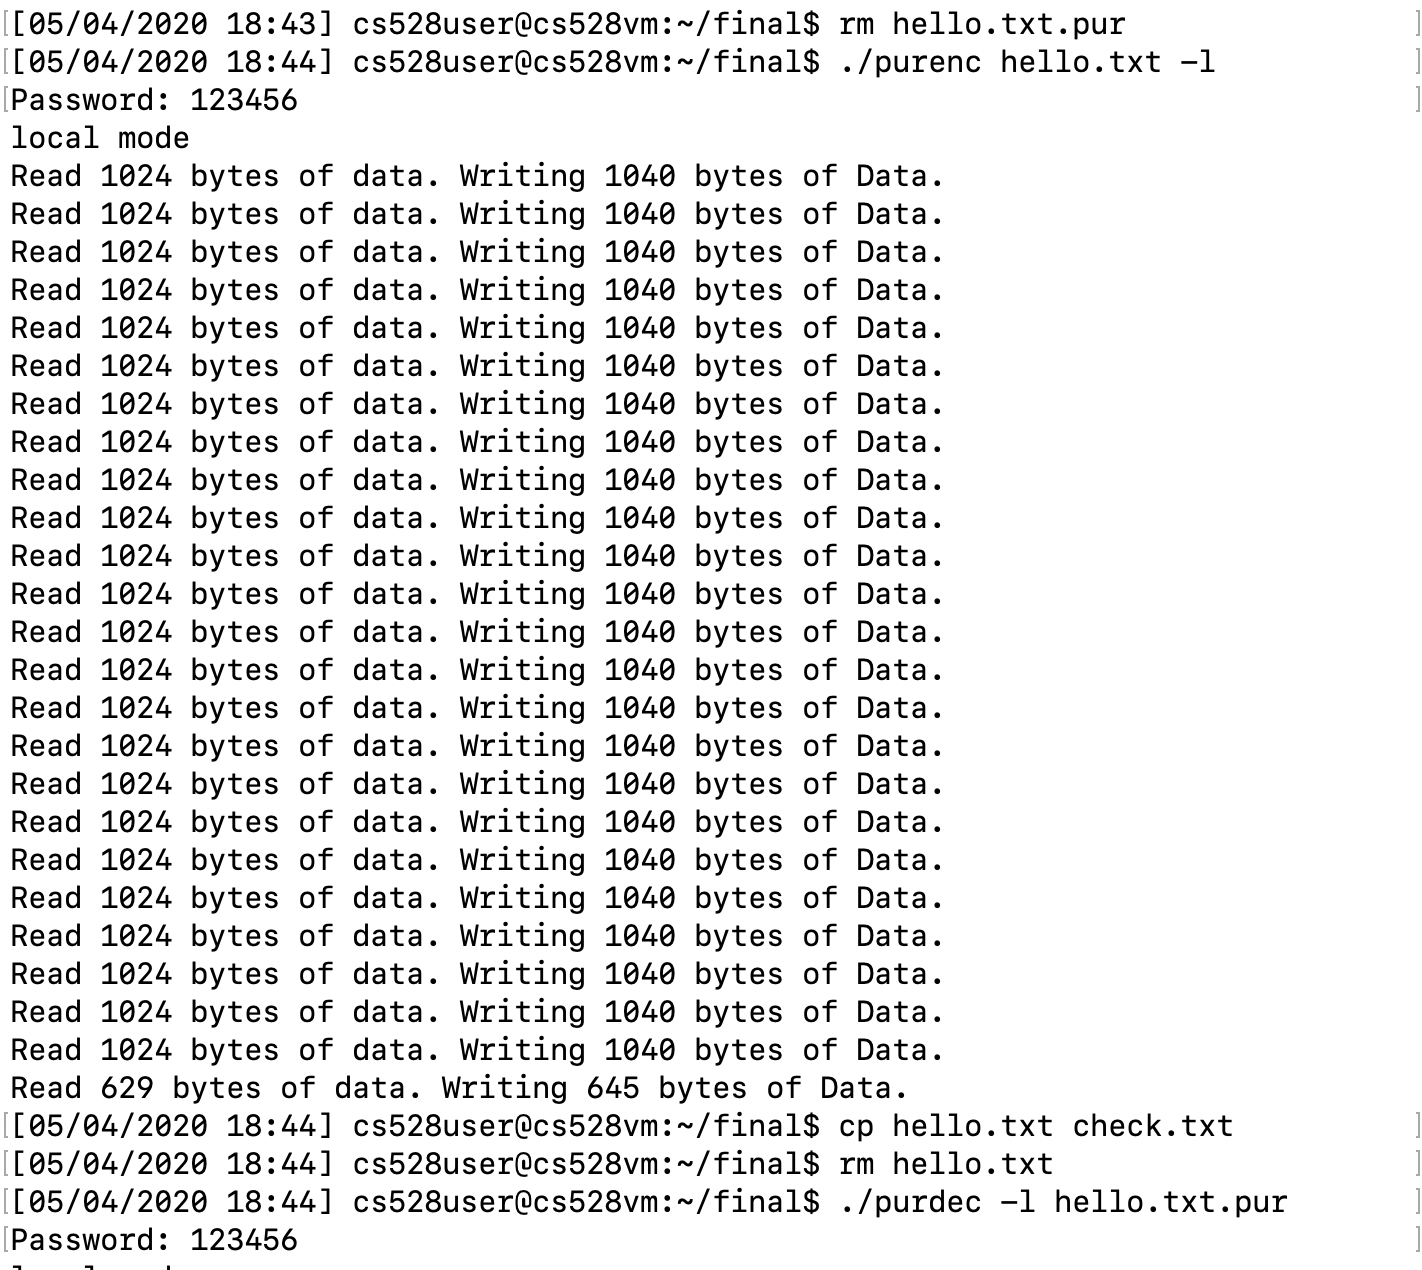
\includegraphics[scale = 0.7]{local1.png} % requires the graphicx package
   \caption{local mode encrpytion}
   \label{fig1}
\end{figure}

Local mode decryption is shown in Fig. \ref{fig2}
\begin{enumerate}
\item decrypt hello.txt.pur to get hello.txt;
\item diff -s hello.txt check.txt. Those files are identical.
\end{enumerate}

\begin{figure}[htbp]
   \centering
   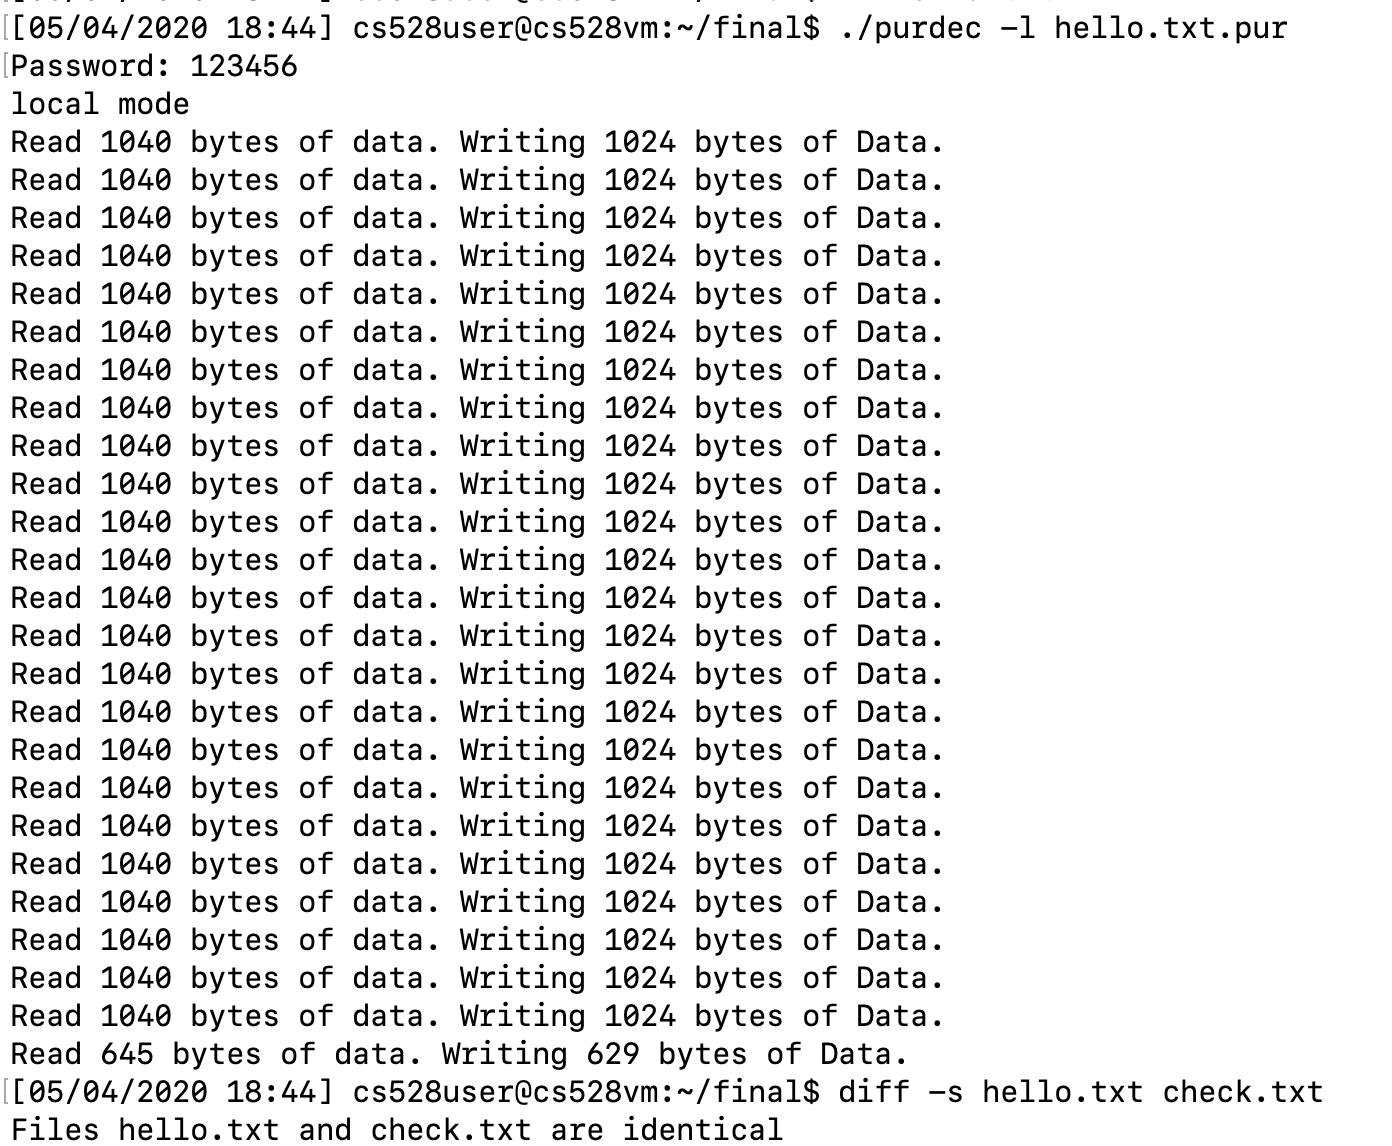
\includegraphics[scale = 0.7]{local2.png} % requires the graphicx package
   \caption{local mode decryption}
   \label{fig2}
\end{figure}

\subsection{distant mode}

Results are shown in Fig. \ref{fig3}. 

distant mode decryption.
\begin{enumerate}
\item copy hello.txt to check.txt;
\item remove hello.txt.
\item receive encrypted file and decrypt it into hello.txt;
\item diff -s hello.txt check.txt. Those files are identical.
\end{enumerate}

\begin{figure}[htbp]
   \centering
   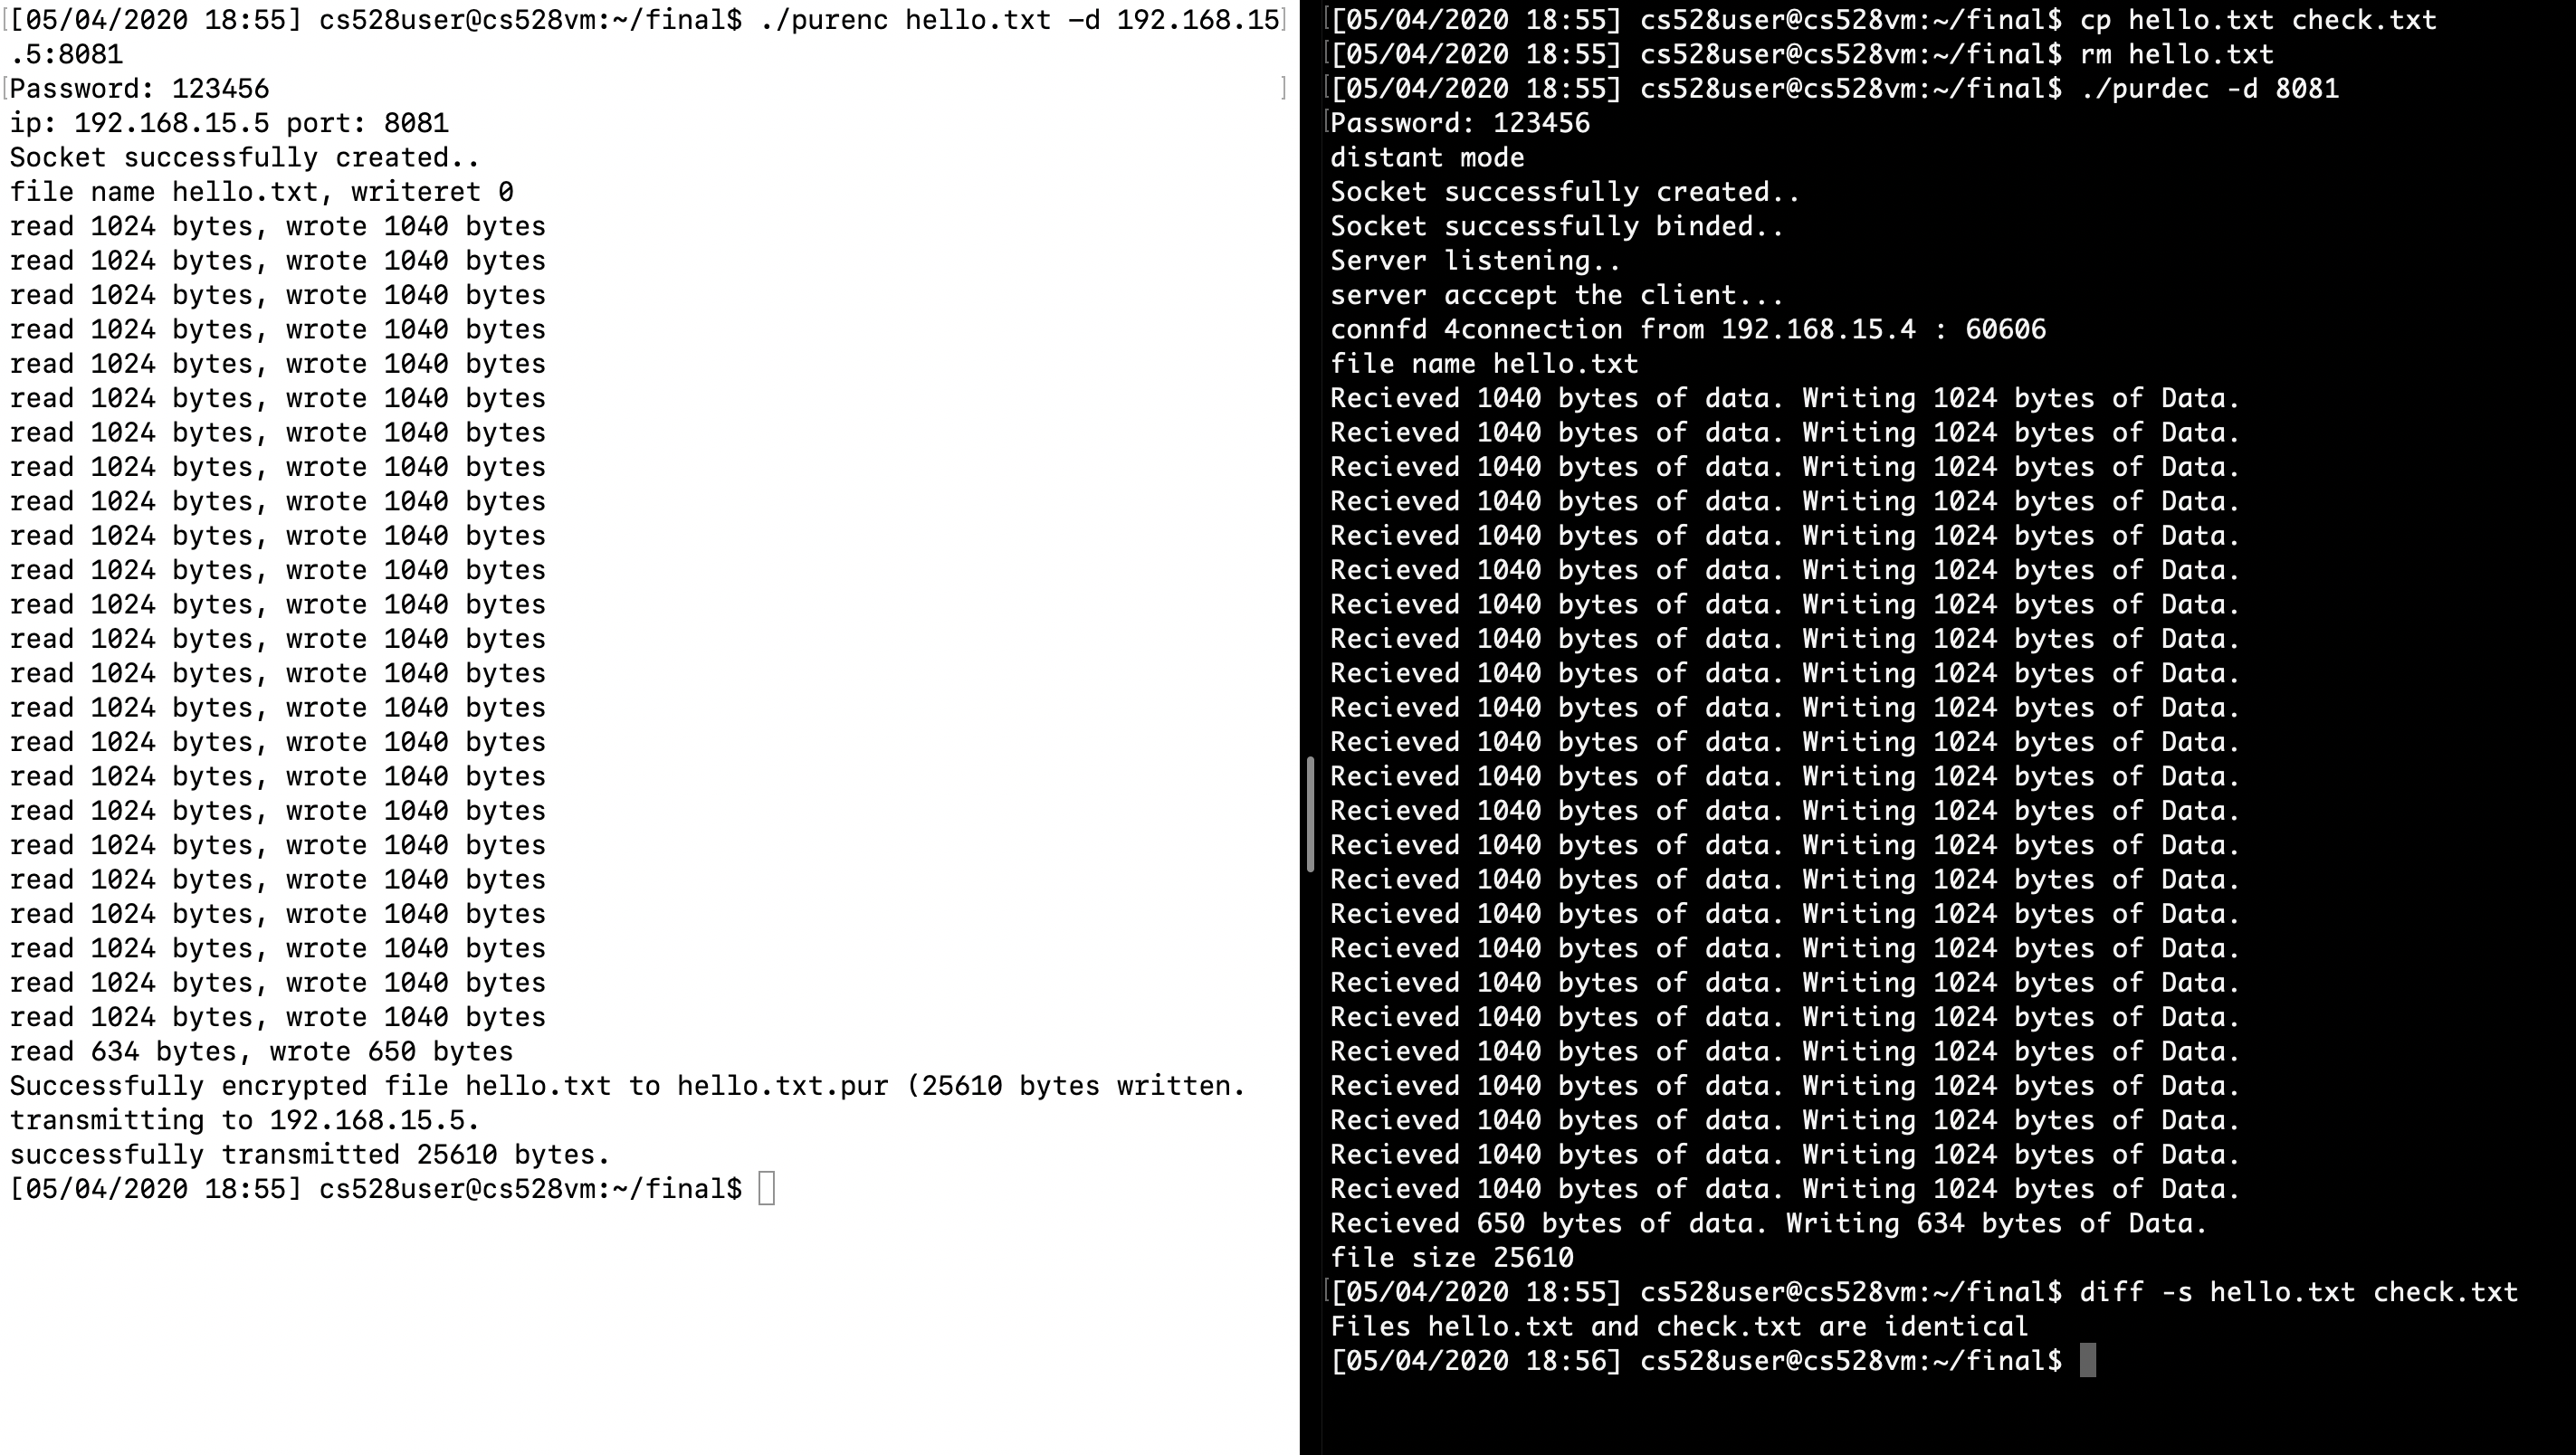
\includegraphics[scale = 0.3]{distant.png} % requires the graphicx package
   \caption{distant mode}
   \label{fig3}
\end{figure}
\end{document}  